% NOTE:
% latexmk -shell-escape -pvc poster.tex # Watches and compiles on each change.
% latexmk -c poster.tex   # Clean the temporal files.


\documentclass[20pt]{beamer}

% Adapted from;
% How to Design a Scientific Poster using Beamer -1 (Latex Basic Tutorial-30)
% https://youtu.be/2ZWnFFhVkdE?si=N3e1Ob8YWyTwW19e

\usepackage[size=custom, width=90, height=120, orientation=portrait, scale=1.4]{beamerposter}
\usetheme{Madrid}
\usepackage{changepage}
\usepackage[numbers]{natbib}
\usepackage{listings}
\usepackage{siunitx}
\usepackage{hyperref}
\usepackage[linesnumbered,algoruled,longend]{algorithm2e}
\usepackage{graphicx}
\usepackage{subcaption}

\beamertemplatenavigationsymbolsempty

\renewcommand{\raggedright}{\leftskip=0pt \rightskip=0pt}
\let\olditemize\itemize
\renewcommand{\itemize}{\olditemize\addtolength{\itemsep}{0.4\baselineskip}}

\addtobeamertemplate{block begin}{}{\vspace{5mm}\begin{adjustwidth}{5mm}{5mm}}
\addtobeamertemplate{block end}{\end{adjustwidth}\vspace{10mm}}{\vspace{5mm}}

\setbeamertemplate{caption}[numbered]

\setbeamerfont{block title}{size={\centering\bfseries\fontsize{48}{60}}}
\setbeamercolor{block body}{bg=white}
\setbeamercolor{background canvas}{bg=white}


\definecolor{rulebg}{RGB}{248,230,0}
\definecolor{titlebg}{RGB}{11,95,156}
\definecolor{titlefontcolor}{RGB}{255,255,255}
\definecolor{rulebg}{RGB}{252,199,21}


\setbeamercolor{fbcolor}{fg=white, bg=titlebg}
\setbeamertemplate{headline}{
    \begin{beamercolorbox}[wd=\paperwidth]{fbcolor}\vskip5mm
        \begin{columns}
            \begin{column}{0.30\linewidth}
            \centering
            
\includegraphics[scale=0.7]{logos/logo_sbsr.png}\\
            \end{column}
            \begin{column}{0.70\linewidth}
                \bfseries
\textcolor{titlefontcolor}{
\fontsize{80pt}{96} 
                \selectfont
                Exploratory analysis of recurrent deforestation \\
                warnings in the Brazilian Amazon\\ [6mm]
{\fontsize{43pt}{60}
                \selectfont 
                Alber Sanchez (alber.ipia@inpe.br), Guilherme Mataveli,
                Luiz E. O. C. Arag\~{a}o }
                }
            \end{column}
        \end{columns}
        \vskip 5mm
    \end{beamercolorbox}
    \color{rulebg}\rule{\paperwidth}{20pt}
}

\setbeamercolor{footcolor}{fg=white, bg=black}
\setbeamertemplate{footline}{
\color{rulebg}\rule{\paperwidth}{20pt}
 \begin{beamercolorbox}[wd=\paperwidth]{fbcolor}\vskip5mm
        \begin{columns}
            \begin{column}{0.30\linewidth}
            \centering
            
\includegraphics[scale=2.5]{logos/logoinpe-azul-menor.png}\\
            \end{column}
            \begin{column}{0.40\linewidth}
                \bfseries
\textcolor{titlefontcolor}{
\fontsize{30pt}{96} 
\centering
                \selectfont
                Acesse o site do grupo:\\ [6mm]
                \vspace{10mm}
                }

\centering
            
\includegraphics[scale=1.8]{logos/trees-color-h_2.png}
                \hspace{10mm}
            
\includegraphics[scale=1.0]{images/qr_treeslab.png}\\
                \vspace{10mm}
            \end{column}
            \begin{column}{0.30\linewidth}
            \centering
            
\includegraphics[scale=1.1]{logos/logo_cnpq.png}\\
            \end{column}
        \end{columns}
    \end{beamercolorbox}
}















\begin{document}\vspace*{-2cm}
\begin{frame}[fragile,t]
\begin{columns}[t]



%==== Column 1 ====

\begin{column}{0.33\linewidth}

\vspace{1cm}

    \begin{block}{Introduction\vphantom{g}}

Current advances in Ecology, Remote Sensing, and Computer Science have enabled the development of regional, continental and global deforestation monitoring systems (e.g., DETER, MapBiomas, Global Forest Watch).
However, detecting and monitoring forest degradation remains more challenging than detecting deforestation~\cite{Lambin:1999,Mitchell2017}.
Given the importance of this issue, here we present the spatial distribution of recurrent forest degradation in the Brazilian Amazon, which could help address the challenges in detecting it. 
We think that deforestation real-time forest monitoring systems, such as DETER that continuously issues deforestation alerts, inadvertently captures forest degradation processes at various stages.
The findings presented here are the results of processing 5 years of DETER alerts.
This paper extends the findings introduced in ~\cite{sanchez2023}.

    \end{block}

\vspace{1cm}

    \begin{block}{Data}
In our analysis, we used DETER data from August 2016 to July 2021.
DETER has produced fast assessments of forest degradation and deforestation in the Brazilian Amazon since 2004~\cite{shimabukuro2006}. 
Figure~\ref{fig:deter_warnings_area_size} show an initial assesment of DETER data.

\begin{figure}[h] 
    \begin{center}
    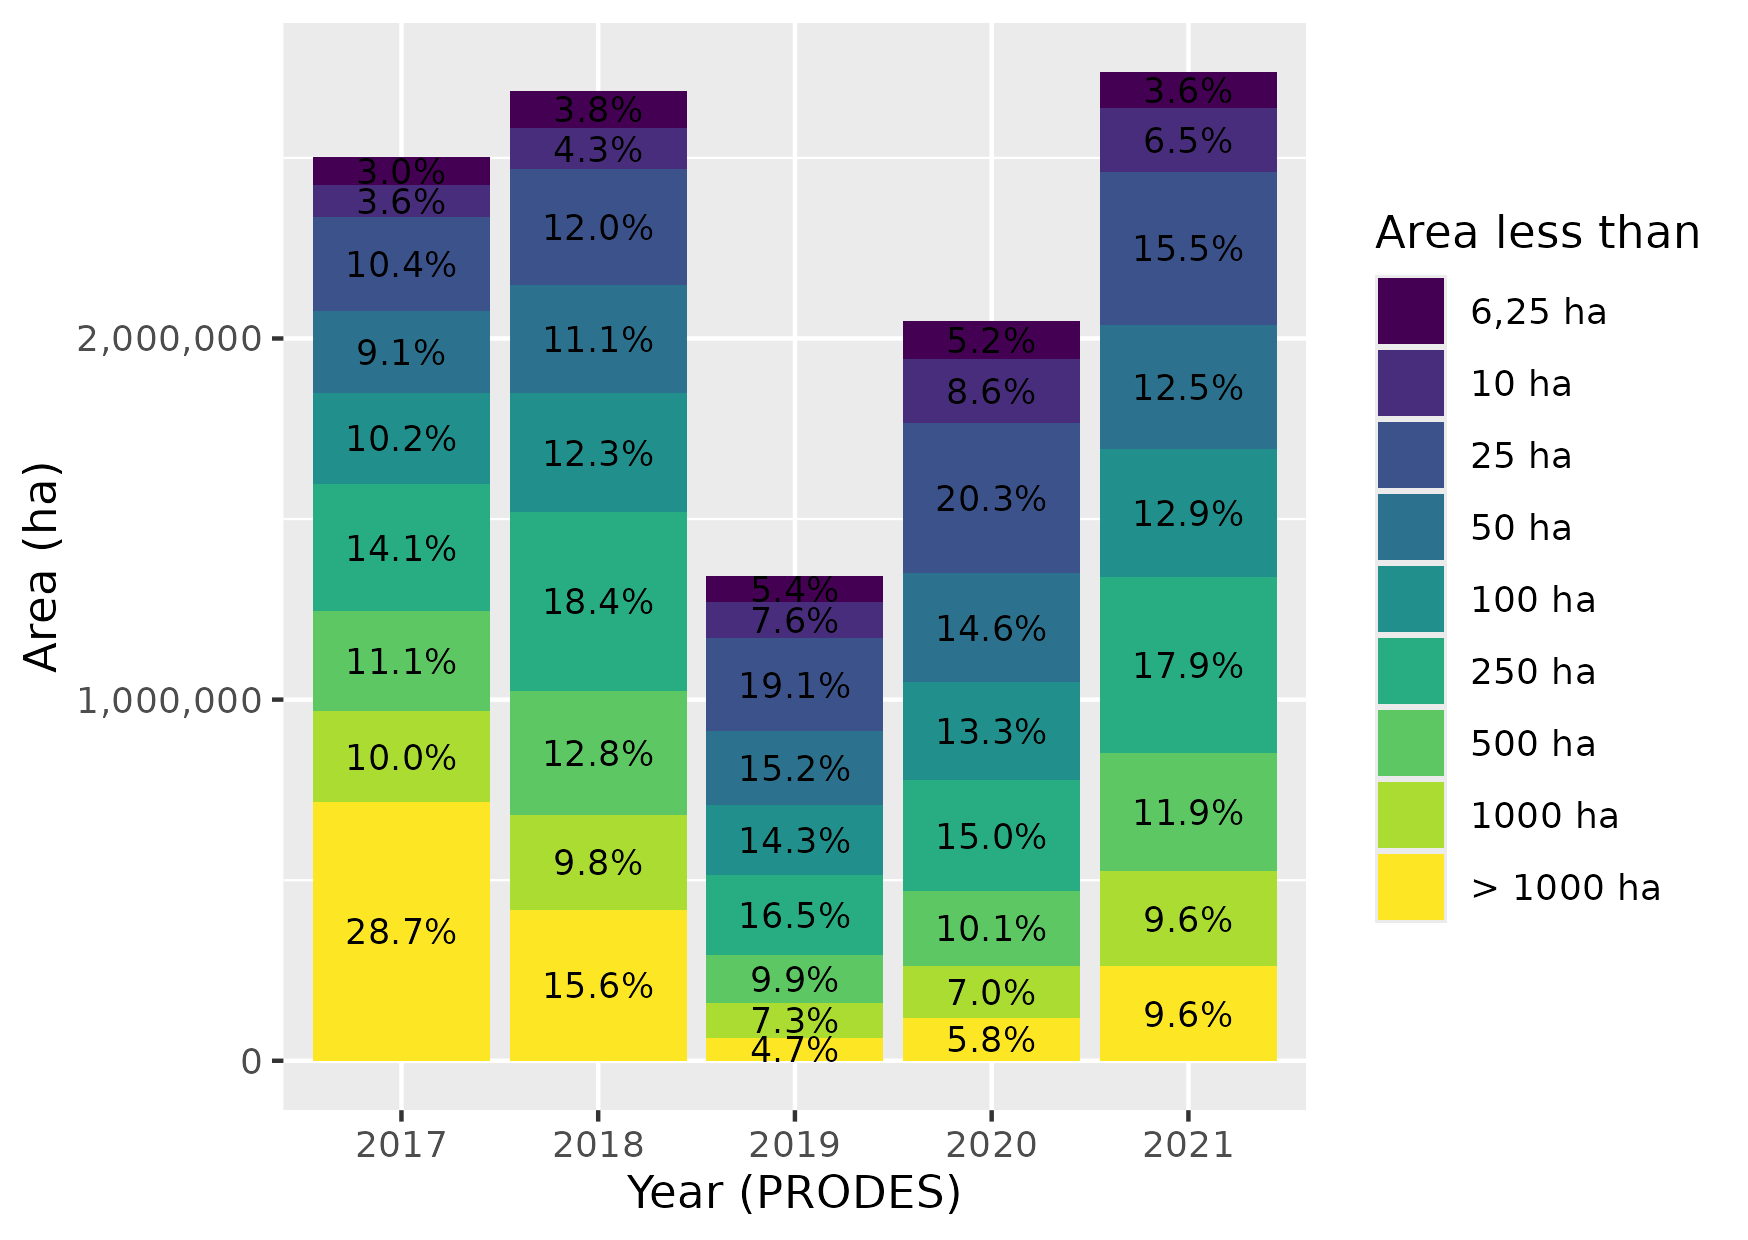
\includegraphics[width=\linewidth]{./figures/deter_warnings_area_size.png}
        \caption{Area of DETER alerts by year and size.
        The total area covered by alerts peaked in 2018 and 2021 while the peak of largest areas was in 2017.
        Note the increasing trend since 2019 and how their area distribution is relatively homogeneous along in 2021.}
    \label{fig:deter_warnings_area_size}
    \end{center}
\end{figure}

% \begin{figure}[h] 
%     \begin{center}
%     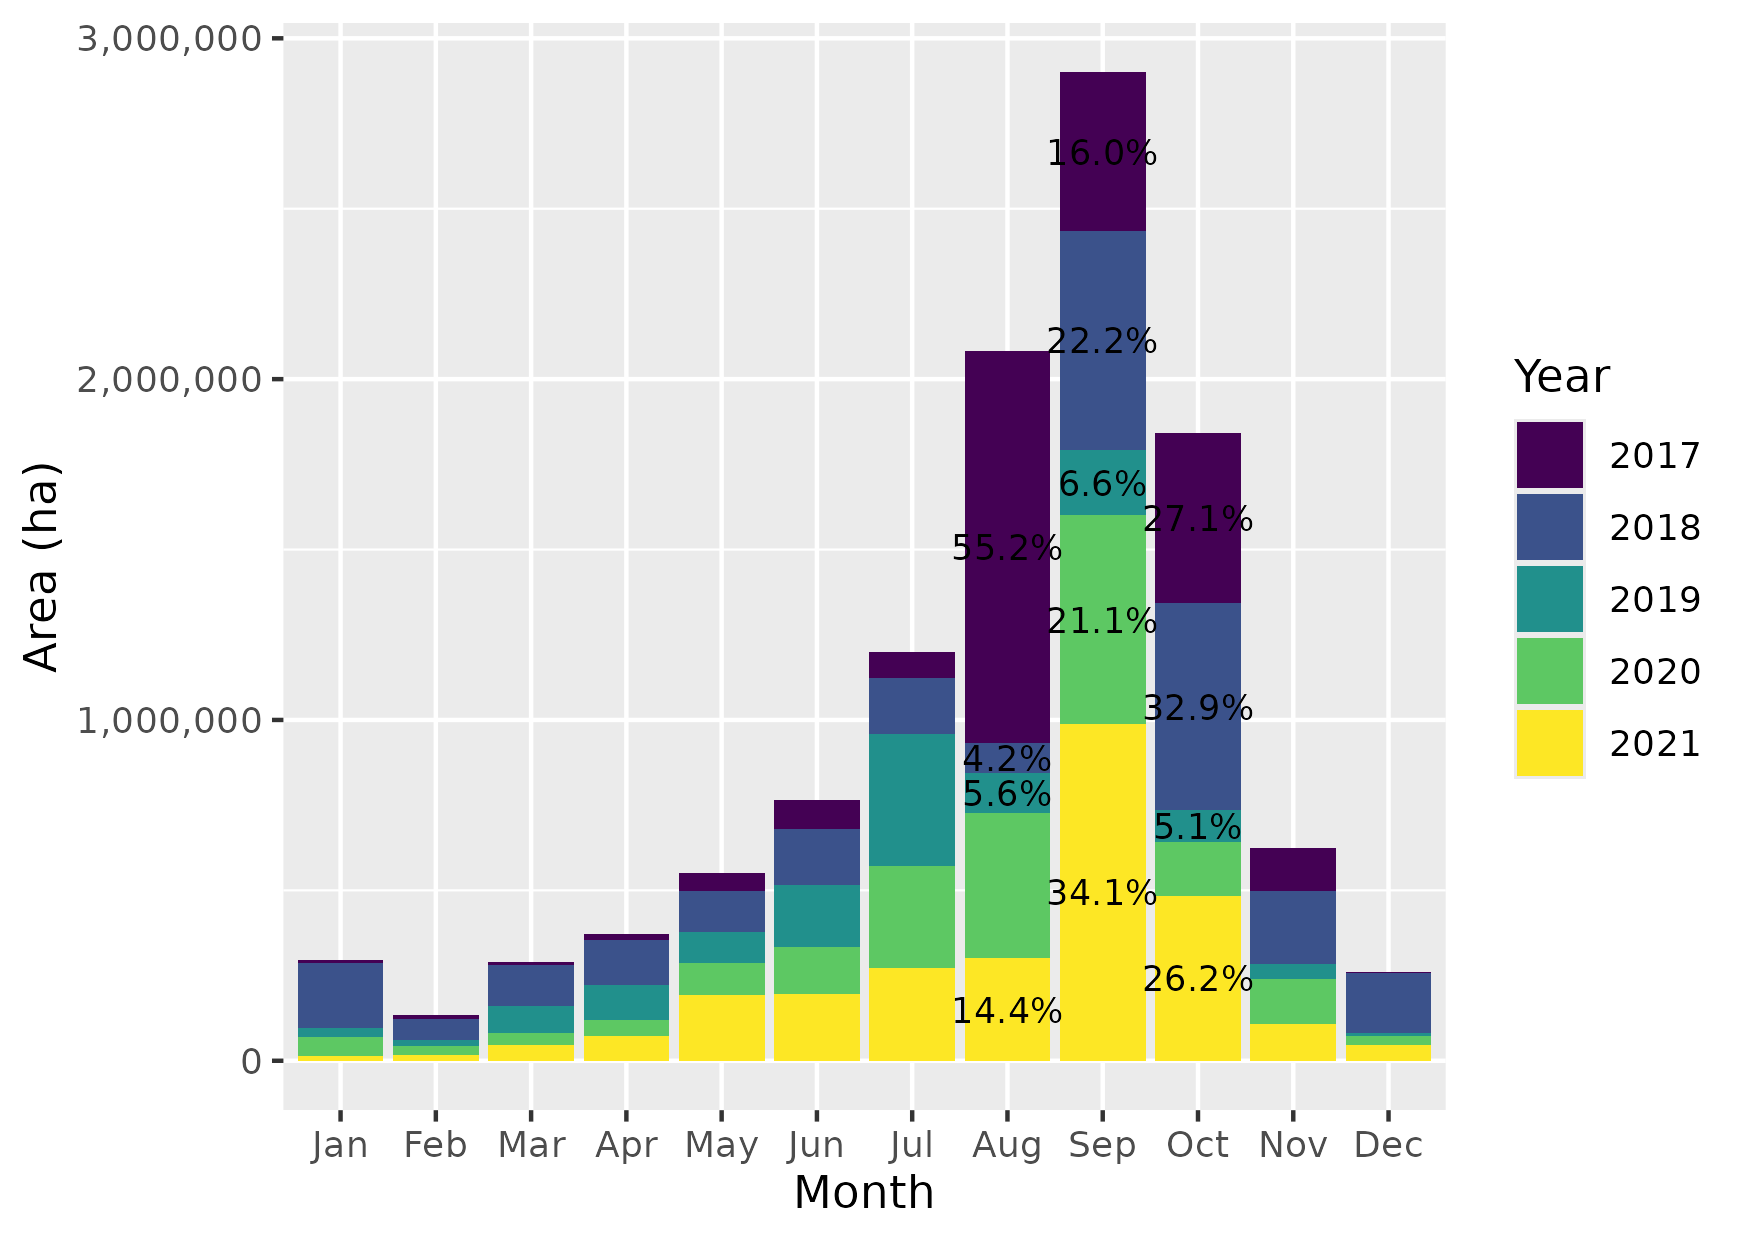
\includegraphics[width=\linewidth]{./figures/deter_warnings_size_month.png}
%     \caption{DETER warnings by month. Between August and October is when most
%         of the warnings are issued. Note how September presents an increasing 
%         trend along the years which peaks in 2021.}
%     \label{fig:deter_warnings_size_month}
%     \end{center}
% \end{figure}

% \begin{figure}[h] 
%     \begin{center}
%     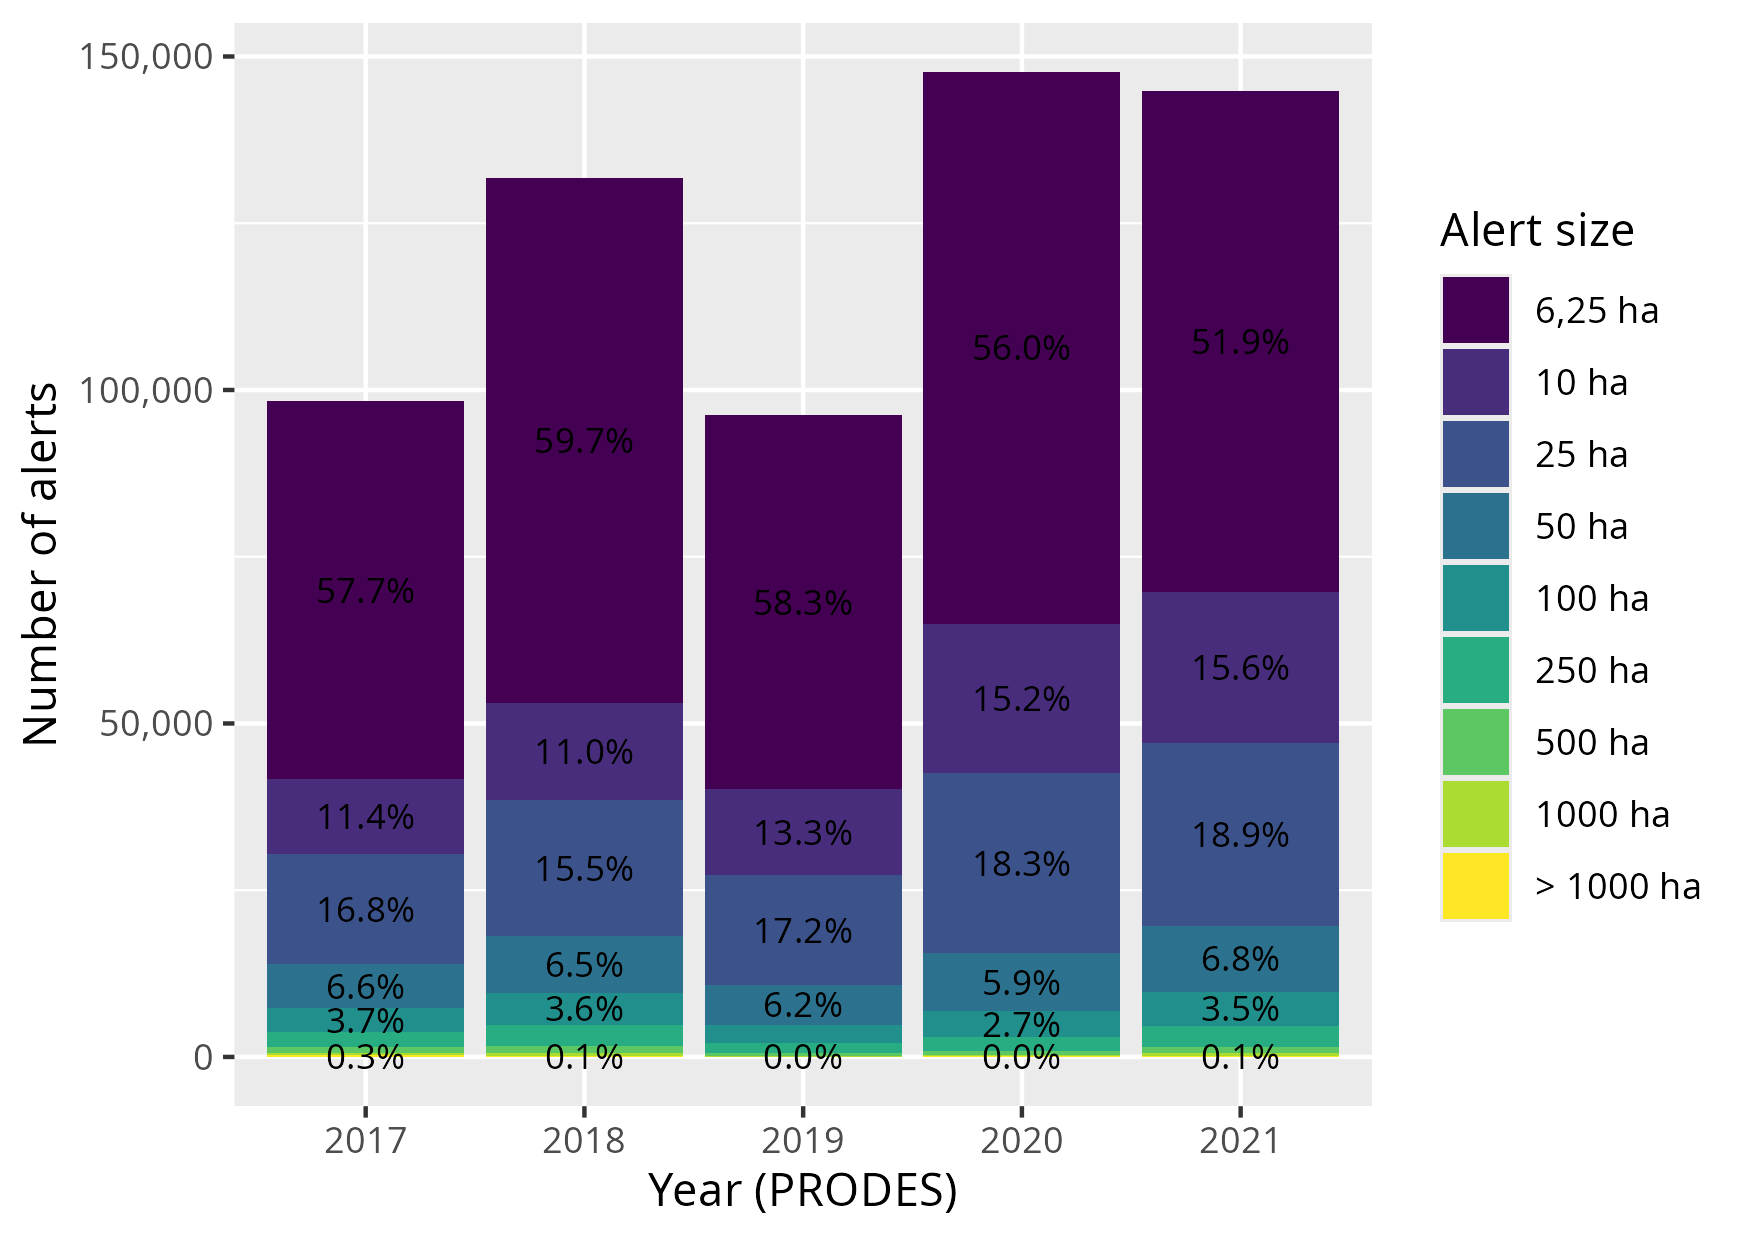
\includegraphics[width=\linewidth]{./figures/deter_warnings_size.png}
%     \caption{Number of DETER alerts by year and size. Note the increasing trend
%         since 2017. Note how DETER issued a similar number of alert in 2020 and
%         2021 but ~Figure~\ref{fig:deter_warnings_size} shows a larger extent of
%         alerts in 2021.}
%     \label{fig:deter_warnings_size}
%     \end{center}
% \end{figure}
    \end{block}

\vspace{1cm}

    \begin{block}{Methods}

        \begin{itemize}
            \item We downloaded DETER data from the TerraBrasilis portal~\cite{f.g.assis2019}. 
            \item Then we self-intersected the data (union operation) and re-projected them to the coordinate reference system UTM 22s.
            \item We removed duplicated vertices and enforced the right-hand rule for polygons, and fixed geometry errors.
            \item We removed alerts smaller than 3~ha.
            \item We computed the PRODES year (August to July).
            \item The results are what we call subareas.
        \end{itemize}

        %This processing was applied using QGIS version 3.38.0~\cite{QGIS_software}.

%This is the reason for the data self-intersection mentioned above.
%The \textit{subareas} resulting from this self-intersection correspond to polygons on which DETER alerts were issued on different dates, and are the base on which our analysis is founded.

%Our analyses were carried out using the GNU's R language and environment for statistical computing and graphics to estimate statistics analysis~\cite{ihaka1996}.
%Our source code is available online.~\footnote{R code available at \url{https://github.com/albhasan/treesburnareas}}

    \end{block}

        \vspace{1cm}

\end{column}



%==== Column 2 ====
\begin{column}{0.33\linewidth}
\vspace{1cm}
    \begin{block}{Results\vphantom{g}}


Moreover, the number of DETER alerts during the same period shows a somewhat similar pattern, characterized by the fact that half of yearly DETER alerts are issued for small areas (Figure~\ref{fig:deter_warnings_size}).

From August to October is when most DETER alerts are issued, and September, the peak month, presents an increasing trend in area, reaching its maximum in 2021.
This period corresponds to the fire season in most of the Brazilian Amazon~\cite{carvalho2021} (see Figure~\ref{fig:deter_warnings_size_month}). 


Most DETER subareas are issued a single alert and never more than five, following an exponential decay pattern.

% \begin{figure}[h] 
%     \begin{center}
%     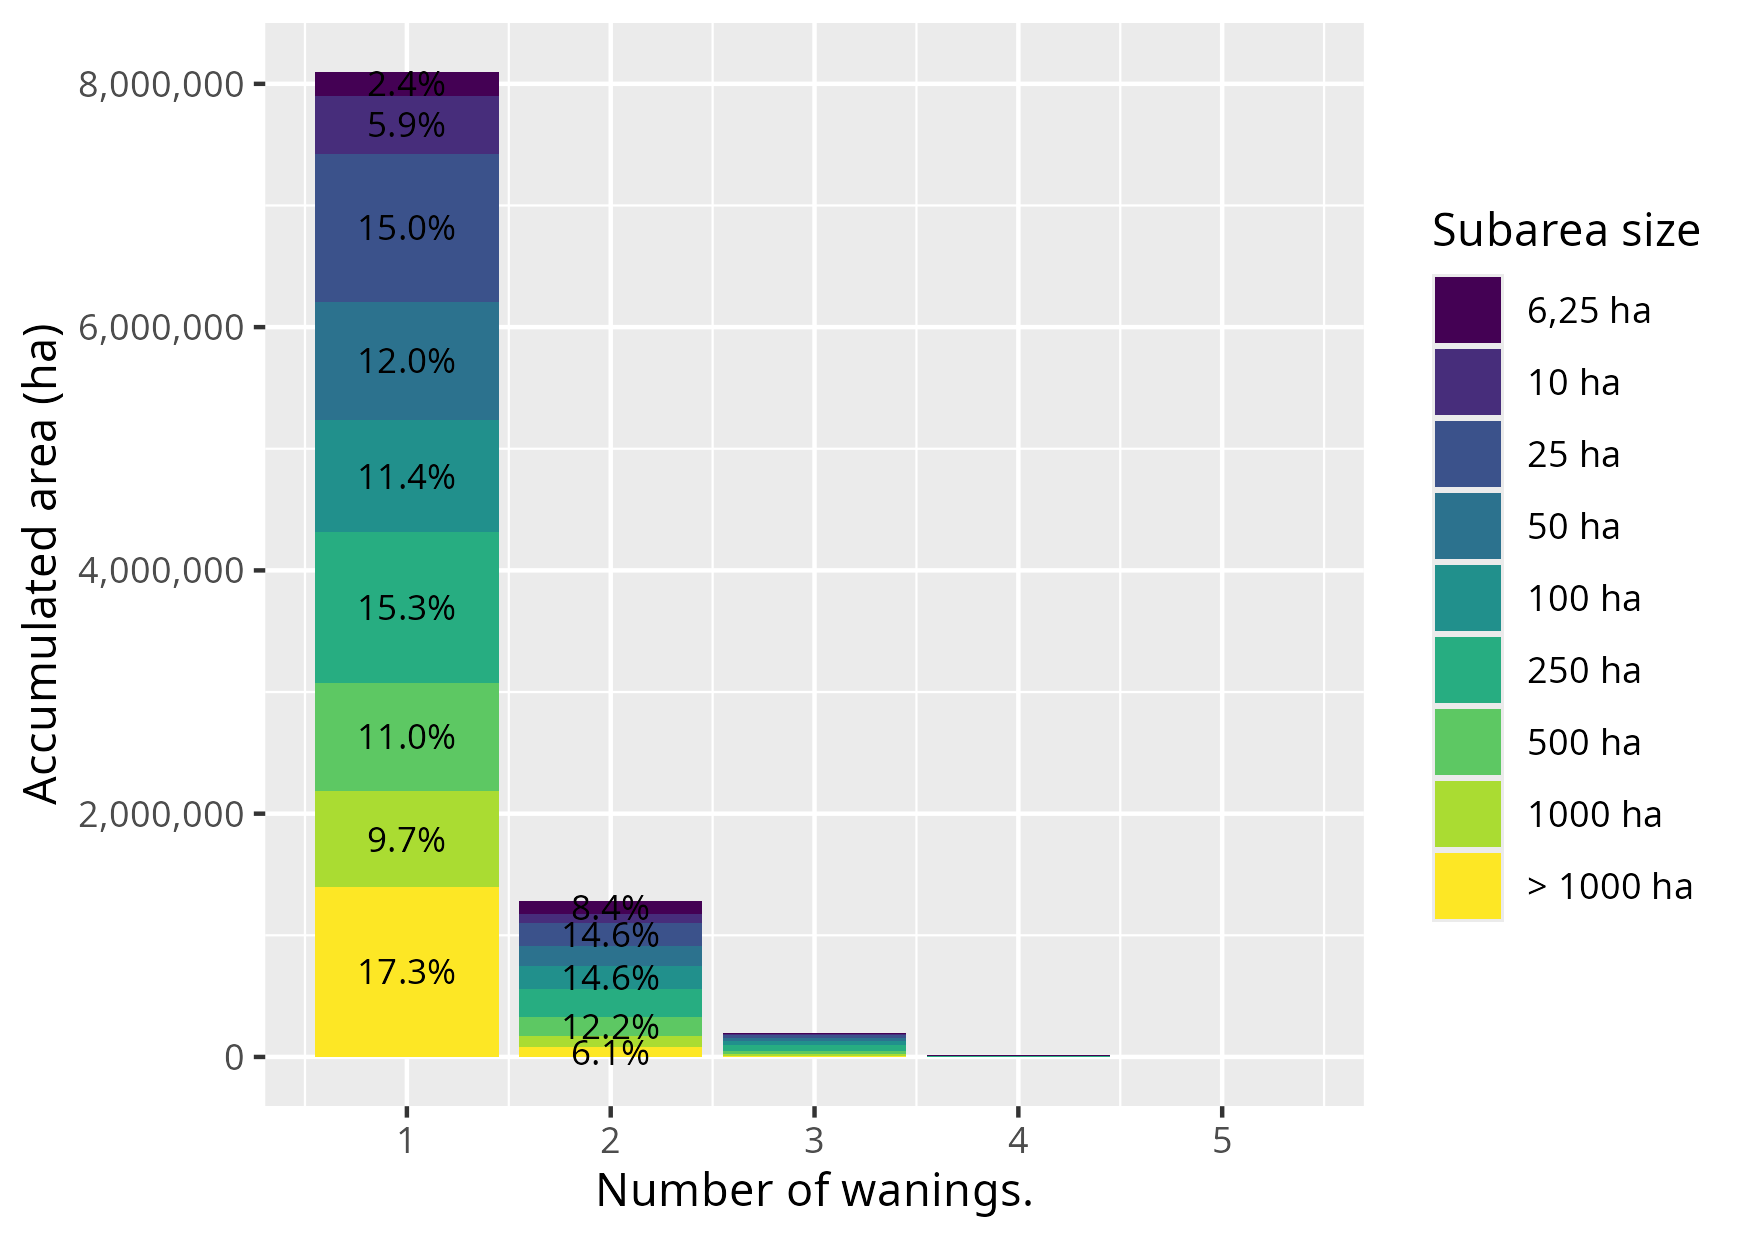
\includegraphics[width=\linewidth]{./figures/plot_area_by_warnings.png}
%     \caption{DETER subareas by number of warnings. Most subareas only have one
%         DETER alert and never more than five. The total extent for each number
%         of alerts is homogeneously distributed.}
%     \label{fig:plot_area_by_warnings}
%     \end{center}
% \end{figure}


The time period between DETER alerts in the same subarea is one year, except for subareas with two alerts, when it is two years (Figure~\ref{fig:plot_days_first_to_last}). 

\begin{figure}[h] 
    \begin{center}
        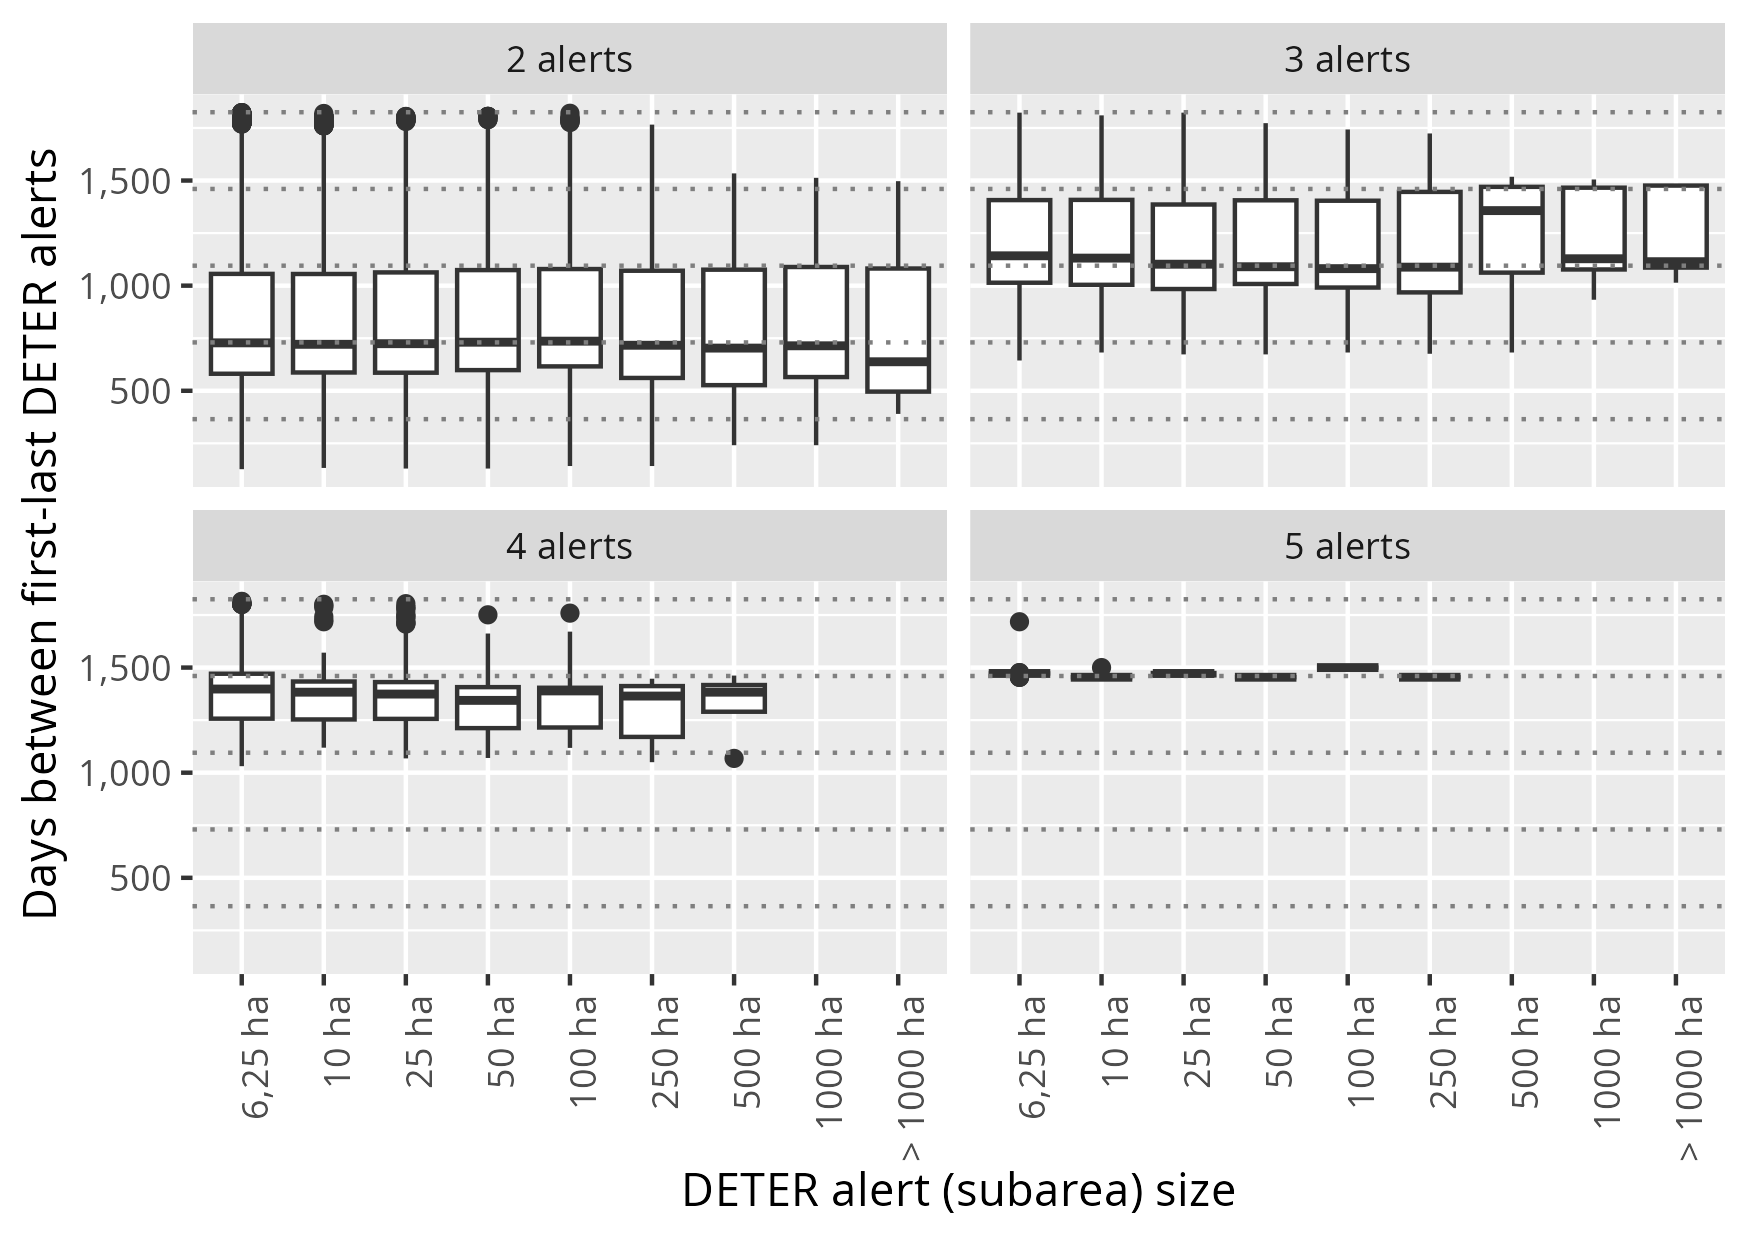
\includegraphics[width=\linewidth]{./figures/plot_days_first_to_last.png}
    \caption{Number of days between the first and last DETER alerts. The
        horizontal dashed black lines represent intervals of 365 days.
        DETER subareas with 2 warnings tend to be two years apart and then
        increase one year with each additional alert. Also note that the
        distribution by area tend to have long tails towards longer periods
        between the first and lat DETER alert.}
    \label{fig:plot_days_first_to_last}
    \end{center}
\end{figure}

The map in Figure~\ref{fig:plot_area_by_warnings} shows the distribution of recurrent deforestation warnings, that is, a surface interpolation of the number of DETER alerts.

\begin{figure}[h] 
    \begin{center}
        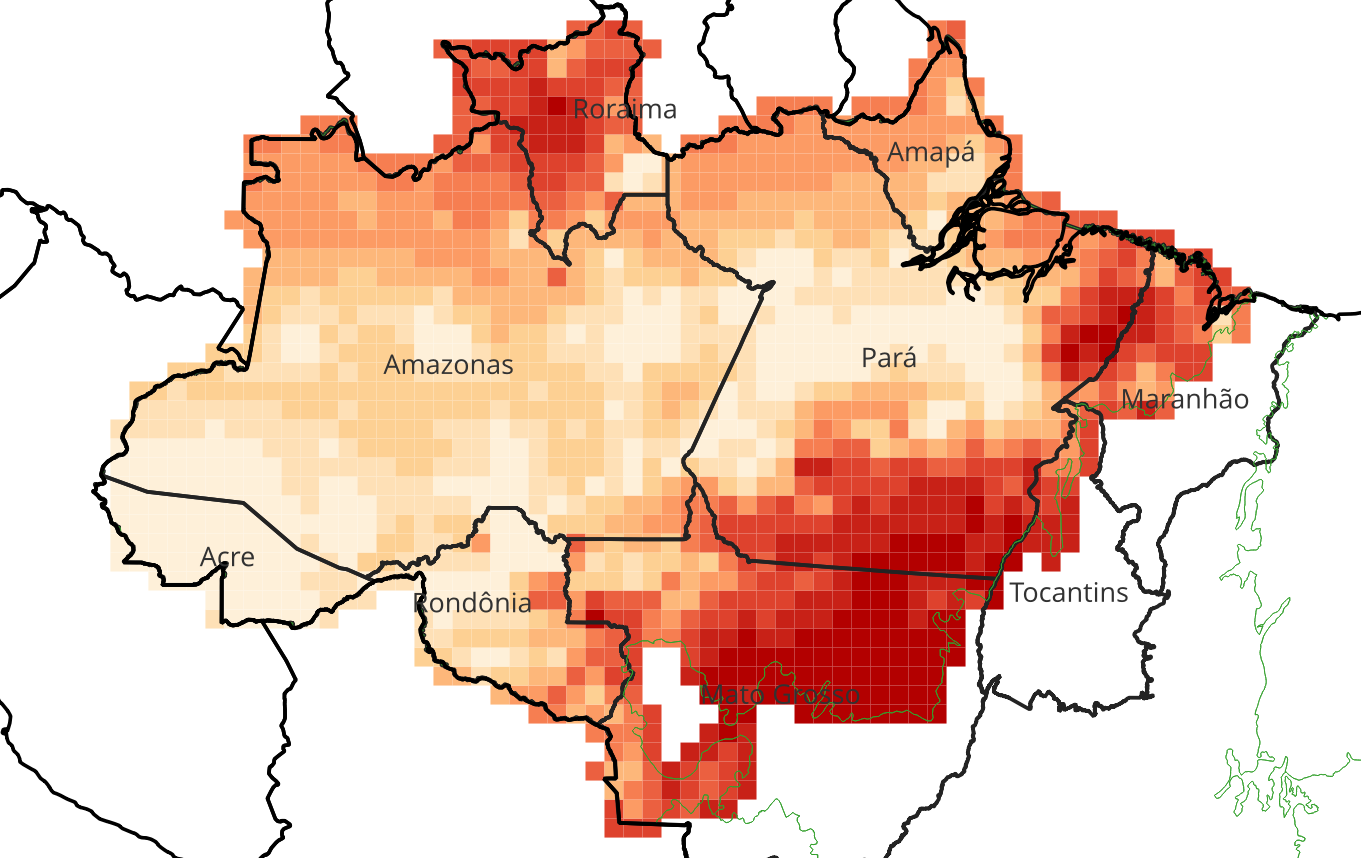
\includegraphics[width=\linewidth]{./figures/nwarnings_idw_map.png}
        \caption{Spatial distribution of recurrent degradation (number of
        alerts by subarea) in the Brazilian Amazon. Amazon's east front is
        where most of recurrent DETER alerts area found.}
    \label{fig:nwarnings_idw_map}
    \end{center}
\end{figure}


    \end{block}
\vspace{1cm}
\end{column}



%==== Column 3 ====

\begin{column}{0.33\linewidth}
\vspace{1cm}
    \begin{block}{Final remarks\vphantom{g}}
        TODO.
    \end{block}

\vspace{1cm}
    \begin{block}{References\vphantom{g}}
    %{\small
\bibliography{sbsr2024}
    %}
\bibliographystyle{sbc}
    \end{block}



\vspace{1.0cm}
    \begin{block}{Links}

\vspace{0.5cm}
\begin{figure}
    \begin{subfigure}[b]{0.2\textwidth}
\centering

\includegraphics[width=0.90\textwidth]{images/qrcode_email_alber_ipia_at_inpe.png}\\
{Email.}
    \end{subfigure}
\end{figure}
\vspace{0.4cm}

\begin{itemize}
\item Email: 
\href{mailto:alber.ipia@inpe.br}{alber.ipia@inpe.br} 
\item Code: {\scriptsize\url{https://github.com/albhasan/prioritizedeforestationhotspots}}
\end{itemize}

    \end{block}
\end{column}


\end{columns}
\end{frame}
\end{document}
